\documentclass{article}
\usepackage[utf8]{inputenc}
\usepackage{fancyhdr}
\usepackage{graphicx}
\usepackage{geometry}

% ---- Commands ------- %
\newcommand{\documentNumber}[1]{
    \LARGE  \textbf{ PUSS2142{#1} } \\
    \medskip
}
\newcommand{\documentVersion}[1]{
    v. {#1}

    \medskip
}
\newcommand{\documentTitle}[1]{
    \centerline{\rule{13cm}{0.4pt}}
    \bigskip \bigskip
    \LARGE \textbf{TimeMate} \\
    \bigskip
    \LARGE {#1} \\
    \bigskip \bigskip
    \centerline{\rule{13cm}{0.4pt}}
}
\newcommand{\documentGroup}[1]{
    \bigskip \bigskip
    \LARGE Group {#1} \\
    \bigskip
}
\newcommand{\documentResponsible}[1]{
    \LARGE Responsible: {#1} \\
    \medskip
}
\newcommand{\documentAuthors}[1]{
    \LARGE Authors: {#1} \\
    \medskip    
}
\newcommand{\documentDate}[1]{
    \date {#1} 
}

\graphicspath{{./images/}} % Defines a path to file images
\renewcommand{\arraystretch}{1.7}  % Vertical padding for tables


% --- Header & Footer ---- %
\pagestyle{fancy}
\lhead{\leftmark}
\rhead{}
\rfoot{\thepage}
\cfoot{}
\lfoot{}


% ------------------------------------------------ #

% ----- FILL THIS ----- %
\title {
    \documentNumber {08}
    \documentVersion {0.2}
    \documentTitle {Project Final Report}
    \documentGroup {2}
    \documentResponsible {Project Management Group}
    \documentAuthors {Project Management group}
    \documentDate {2021-03-18}
}

\begin{document}

\maketitle
\thispagestyle{empty}

\newpage

\tableofcontents

\newpage

\section{Document History}
\begin{tabular}{ l | l | l | l }
    Version & Date & Responsible & Description \\
    \hline
    0.1 & 2021-03-17 & PG & Document created. \\
    \hline
    0.2 & 2021-03-19 & PG & Ready for informal review. \\
\end{tabular}

\section{Terminology}
    
    See table \ref{Terminology}.
    
    \begin{table}[h]
        \centering
        \begin{tabular}{| l | l |}
            \hline
                SG & System management Group \\
            \hline
                DG & Developer Group \\
            \hline
                TG & Test Group \\
            \hline
                PG & Project Management Group \\
            \hline 
                SDP & Software Development Plan \\
            \hline
                SRS & Software Requirements Specification \\
            \hline
                SVVS & Software Verification and Validation Specification \\
            \hline
                SVVI & Software Verification and Validation Instruction \\
            \hline
                STLDD & Software Top Level Design Document \\
            \hline
                SVVR & Software Verification and Validation Report \\
            \hline
                SSD & System Specification Document \\
            \hline
        \end{tabular}
        \caption{Terminology}
        \label{Terminology}
    \end{table}

\section{Referenced Documents \label{refs}}
    \begin{itemize}
        \item Software Development Plan, v. 1.1, Doc. number: PUSS214200.
        \item \label{PH} Project Instruction (Projekthandledningen).
    \end{itemize}

\newpage

\section{Executive Summary}
    This report summarises the work done by project group 2 in the course \emph{Programvaruutveckling för stora projekt}. The project took took place during January, February and March of 2021. It involved 21 students and 3 faculty members at Lund University. The aim of this project was to give students practical experience of working in a large group to produce a time reporting software. Whilst the a time-reporting software was the end product, this report mainly focuses on the lessons learned during the course of the project. The group delivered a product that met the requirements within the allotted time space and considered a success.
    \\ \\
    This report is structured as the following: Section \ref{overview} gives an historic overview of the
    project, section \ref{analysis} aims to analyse the result and reason why certain actions occured
    and how to prevent them. Section \ref{tips} gives six tips for future project groups and lastly section \ref{conclusion} presents a conclusion of the project.

\section{Project Overview \label{overview}}
    This section aims to give an overview of the project and is structured as the following:
    Section \ref{phase1} to \ref{phase4} describes the work process for each phase as well as how they turned out. Figures are included which displays the reported time from each member of the group. Section \ref{reported_time} to \ref{system_locally} does not belong to a specific phase, but rather describes how certain aspects of the project turned out. 
    \\ \\
    The project officially started on week 3 and lasted until the end of week 11.
    
    \subsection{Phase 1. Week 3-5 \label{phase1}}
        PG started planning and gathering the group during week 2 to prepare for phase 1.
        The first phase was a bit of a scramble as people tried to 
        figure out their role, what all the documents where for, how github worked and what latex is. 
        In other words, there was a lot of new information to take in.
        \\ \\
        Writing the SDP, SRS and SVVS, which would lay the ground work for the next few months, went quite well. The first informal
        review failed to catch most of the critical errors, which led to the formal reviewer not approving the documents for baseline. 
        After reworking the documents, and our review process, we held a second informal review. This time around, the remarks where 
        significantly more useful but the structure of the meeting didn't support the ensuing discussions. During the transition 
        into phase 2 we took what we had learned and made some adjustments to our review methods.
        \\ \\
        Writing the SDP, SRS and SVVS, which would lay the ground work for the next few months, went quite well. 
        The main reason for the delay was that the formal review resulted in quite a few changes. This was 
        due to our informal review not catching most of the flaws in our documents. The reasons for why that was and 
        how we corrected for it is detailed in the analysis section. 
        \\ \\
        \begin{figure}[!htb]
            \minipage{0.32\textwidth}
              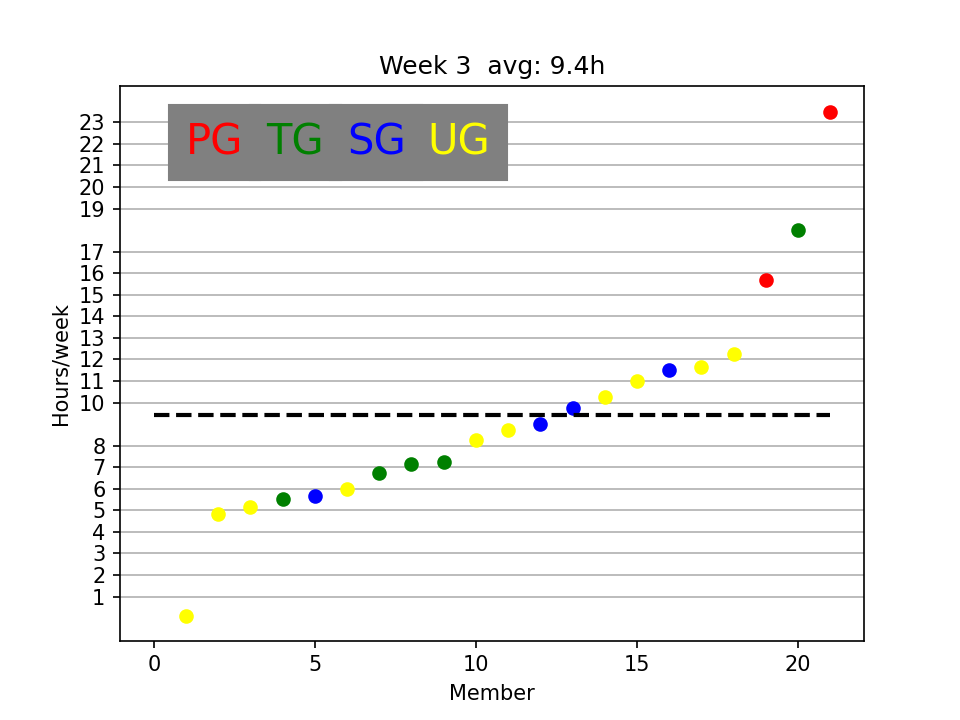
\includegraphics[width=\linewidth]{images/week_3.png}
              \caption{Worked hours week 3}\label{fig:week3}
            \endminipage\hfill
            \minipage{0.32\textwidth}
              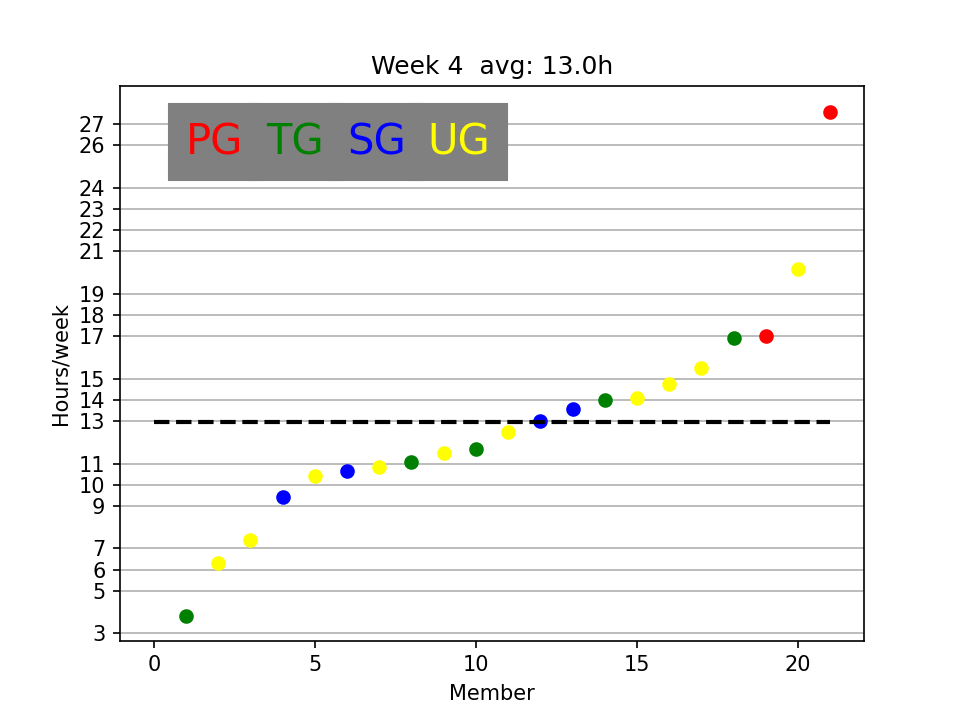
\includegraphics[width=\linewidth]{images/week_4.png}
              \caption{Worked hours week 4}\label{fig:week4}
            \endminipage\hfill
            \minipage{0.32\textwidth}%
              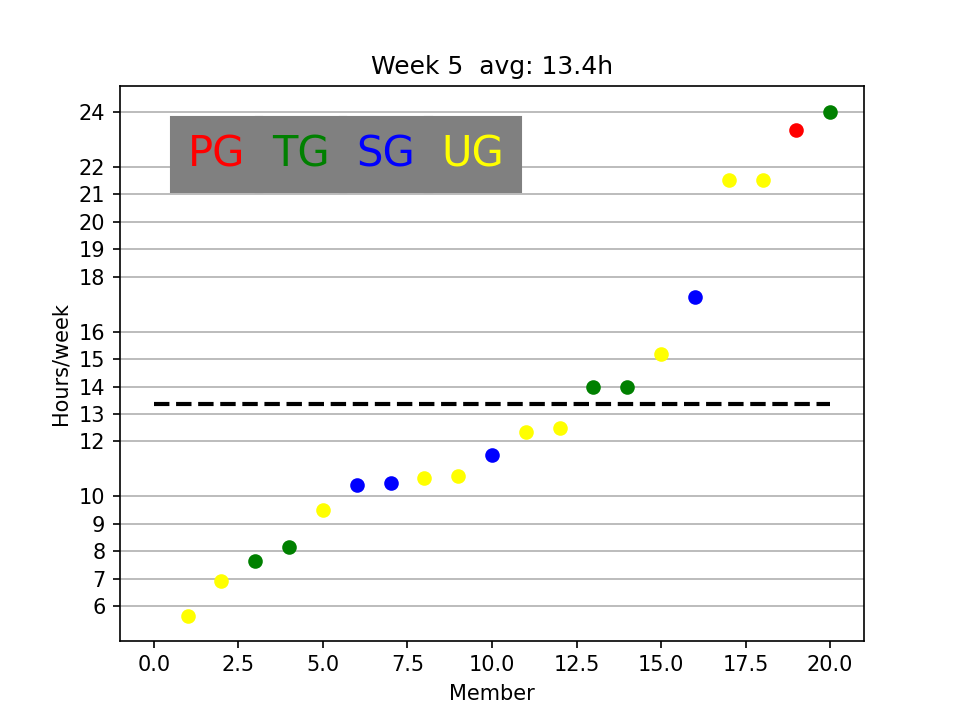
\includegraphics[width=\linewidth]{images/week_5.png}
              \caption{Worked hours week 4}\label{fig:week5}
            \endminipage
        \end{figure}

    \subsection{Phase 2. Week 6-7 \label{phase2}}
        Due to the delay at the end of phase 1, the second phase was compressed to stay on schedule. 
        There was a slight panic at the beginning of the phase as the document deadline was closer than some group 
        members had anticipated. This was solved with some swift scheduling and effective work distribuition within 
        the DG. They scheduled an extra work shift and dedicated 3 members to doing graphics for 
        the STLDD, which helped pipeline the writing process. DG had spent some time during phase 1 preparing for 
        this document, which helped them get started with writing.
        \\ \\
        The writing of SVVI went straight forward as TG was very focused throughout the phase. 
        \\ \\
        The formal review went well. The reviewer had a few remarks, but left it up to us to correct them and put the 
        documents in baseline. A couple of members from TG and DG where tasked with doing this, whilst the others started 
        with development and testing. Getting a head start in the next phase whilst others finished up the current phase 
        became a common strategy, even if it contradicted the strict rules outlined in the waterfall method. 
        
        \begin{figure}[!htb]
            \minipage{0.16\textwidth}
            \endminipage\hfill
            \minipage{0.32\textwidth}
              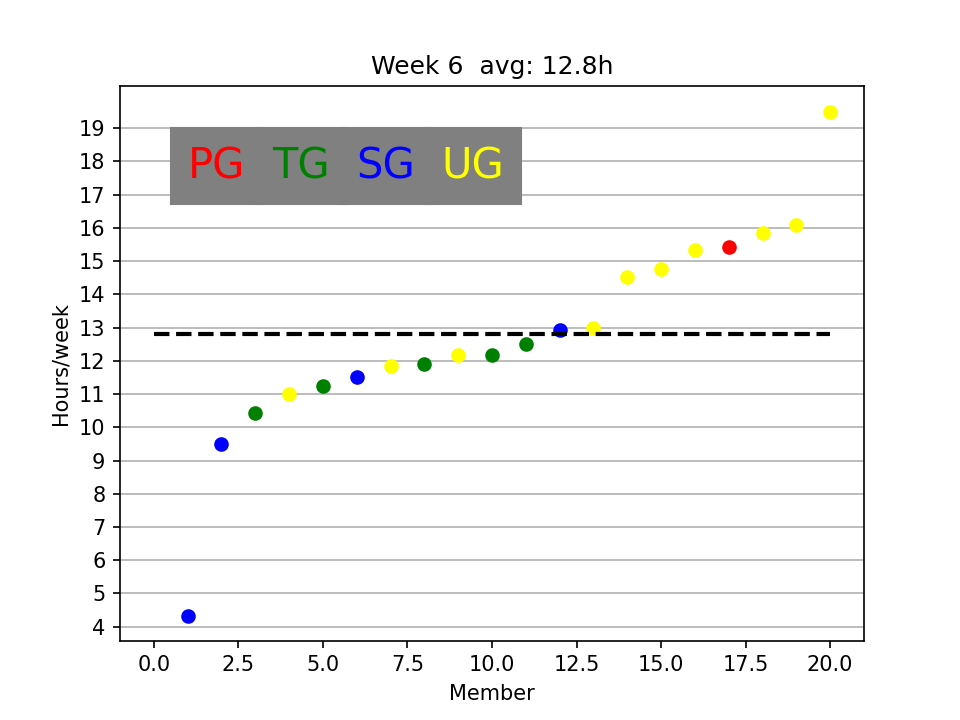
\includegraphics[width=\linewidth]{images/week_6.png}
              \caption{Worked hours week 6}\label{fig:week6}
            \endminipage\hfill
            \minipage{0.32\textwidth}
              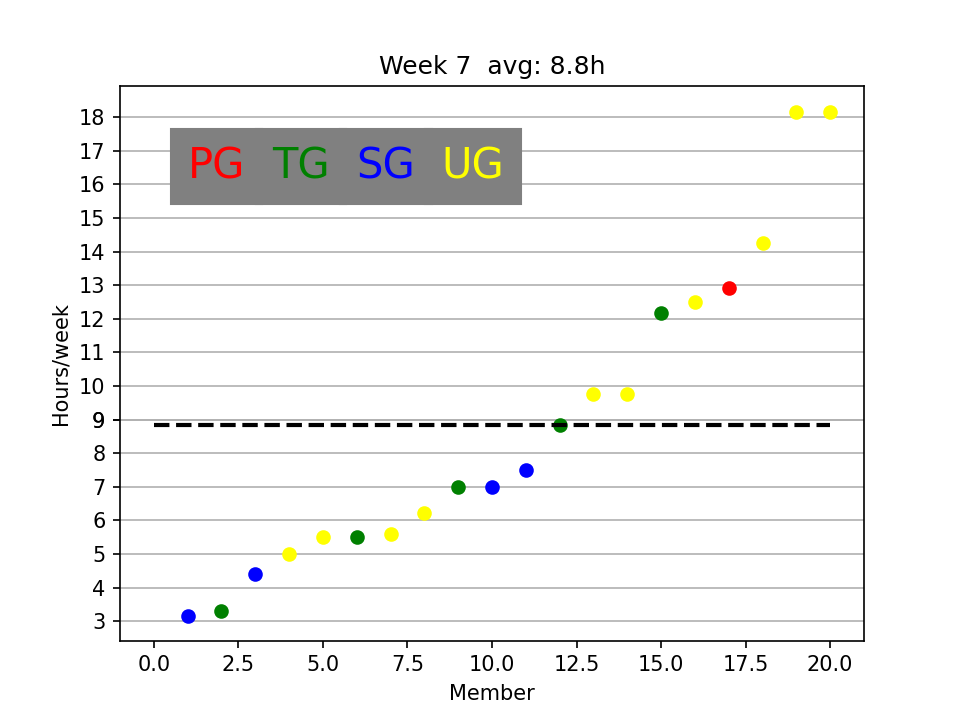
\includegraphics[width=\linewidth]{images/week_7.png}
              \caption{Worked hours week 7}\label{fig:week7}
            \endminipage\hfill
            \minipage{0.16\textwidth}
            \endminipage\hfill
        \end{figure}
        
    \subsection{Phase 3. Week 8-9 \label{phase3}}
        Phase 3 \emph{unofficially} started on time, but \emph{officially} three days late, due to 
        the formal review result in Phase 2. This meant that the group had roughly a week to finish all 
        the code before the first informal review. This caused some panic and many memebers
        did not believe that the deadline would be reached.
        \\ \\
        DG spent a lot of time trying to translate the contents of STLDD to practical code 
        and ambiguities started to show regarding how the system was suppose to fit together.
        This meant that valuable time that should have been spent producing running code, was
        instead speant on understanding the STLDD as well as the SRS. This lead to the existence 
        of \emph{heroes} that put in considerably more hours than others, as seen in figure \ref{fig:week9}.
        \\ \\
        Uncertainties regarding the purpose and responsibilites of SG was somewhat unclear became very obvious
        during this phase. The initial plan was that SG was supposed to aid DG and handle the communication
        between DG and TG and assist any of the groups if needed. It seemed like there were either a 
        missunderstanding of this, or a lack of communication between SG and the rest, because according 
        to SG, no one needed help, but in reality, DG was quite far behind even early in phase 3.
        \\ \\
        The informal review was pushed forward a day and reviewing of code
        convention and code style was ignored due to such "unfinished" code. Instead, only
        functional tests and system tests were reviewed, which all passed. However, there
        were still minor deviations in the system compared to the SRS as well as plenty of 
        undocumented and ugly code. 
        \\ \\
        The second informal review was pushed from Friday to Tuesday week 10, which was enough
        for the group fix the corrections. After this review, further fixes were required,
        such as deleting unused variables and missing javadoc comments. Corrections were made
        and on Friday week 10 phase 3 reached baseline.
        
        \begin{figure}[!htb]
            \minipage{0.16\textwidth}
            \endminipage\hfill
            \minipage{0.32\textwidth}
              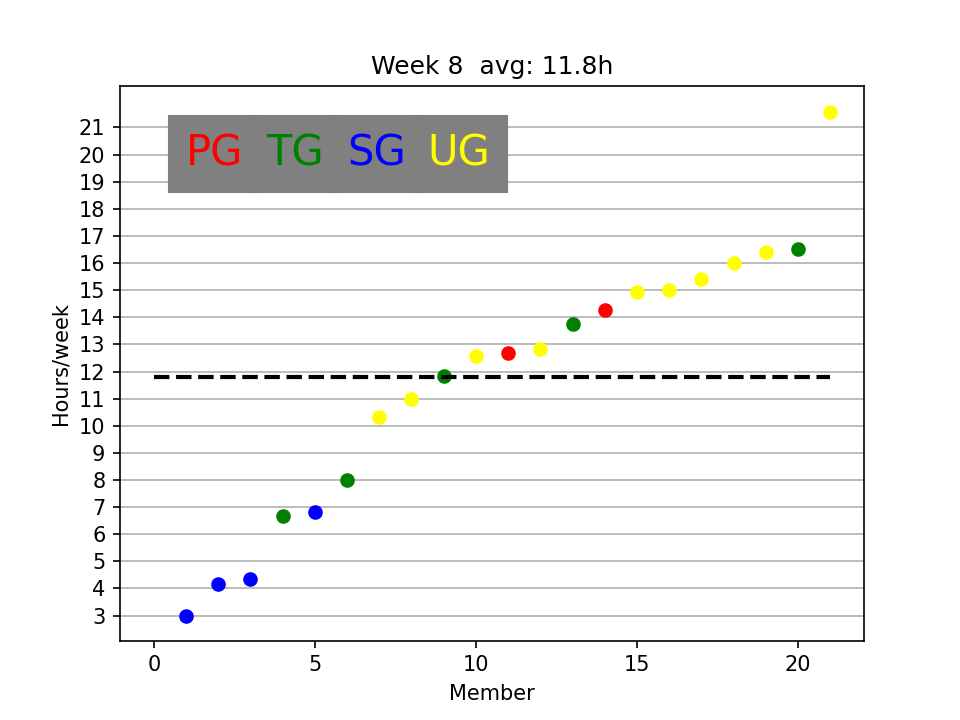
\includegraphics[width=\linewidth]{images/week_8.png}
              \caption{Worked hours week 8}\label{fig:week8}
            \endminipage\hfill
            \minipage{0.32\textwidth}
              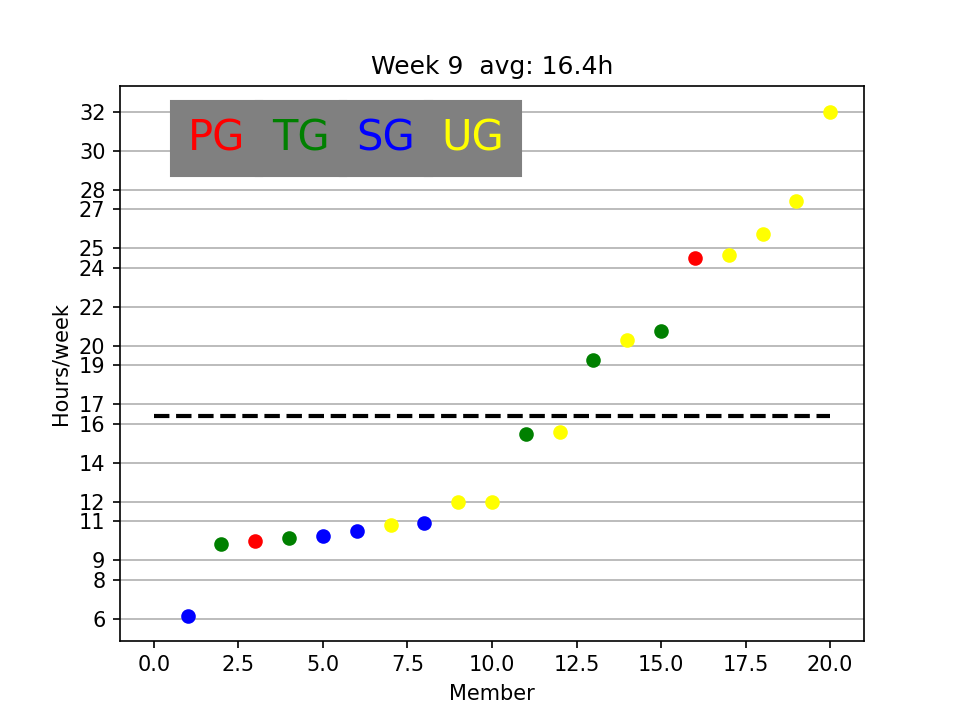
\includegraphics[width=\linewidth]{images/week_9.png}
              \caption{Worked hours week 9}\label{fig:week9}
            \endminipage\hfill
            \minipage{0.16\textwidth}
            \endminipage\hfill
        \end{figure}
        
        
    \subsection{Phase 4. Week 10-11 \label{phase4}}
        Once phase 3 had reched baseline the group took a break from the project and instead
        focused on studying for other exams (week 11 was exam week). However, certain parts
        of phase 4 were already almost done during phase 3 such as SSD, SVVR and the demo
        for the Acceptance meeting. 
        \\ \\
        The last project group meeting was in week 11 and informal review for phase 4 on 
        Friday week 11. Figure \ref{fig:week10} clearly shows that the project was \emph{not}
        in focus and week 11 is spent writing this report so the graph is not included.
        \begin{figure}[!htb]
            \centering
            \minipage{.32\textwidth}
              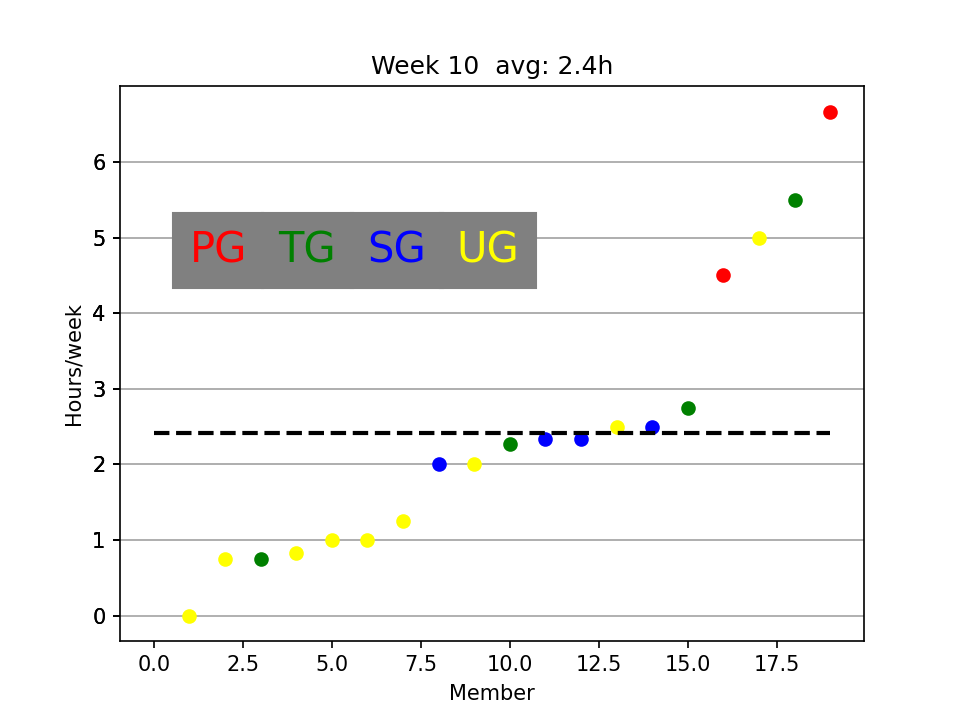
\includegraphics[width=\linewidth]{images/week_10.png}
              \caption{Worked hours week 10}\label{fig:week10}
            \endminipage\hfill
        \end{figure}

    \subsection{Reported Time \label{reported_time}}
        Figure \ref{fig:final} illustrates the average worked hours/week for each phase.
        This number (9.8h/week) is very close to the expected value stated in SDP which was 10
        hours per week. However, even though the \emph{average} hours worked during the project came out to be 
        almost exactly what was expected, it is clear from figure \ref{fig:week3} to \ref{fig:week10}
        that the hours were \emph{not} evenly distributed. Clear hereos started to show early
        on and while this was discussed as a potential risk early in the project, it seemed unavoidable.
        After week 5, PG showed graphs from reported work time to point out the differences and 
        invited the people who had spent less time to spend more, and to the ones who spent more time,
        to spend less as well as ask for help. 
    
        \begin{figure}[!htb]
            \centering
            \minipage{.32\textwidth}
              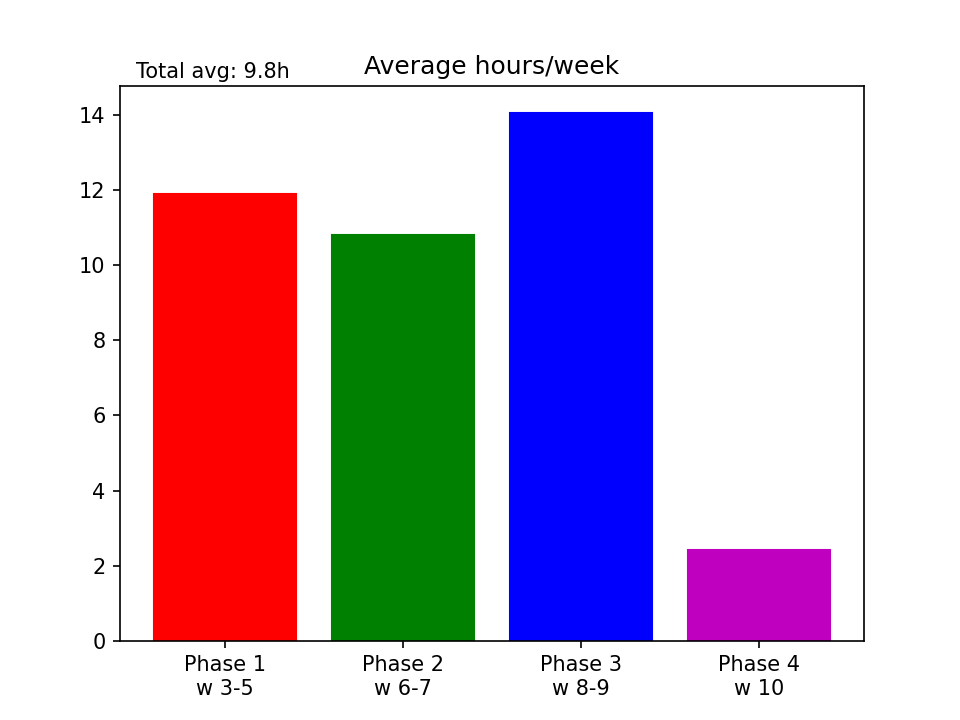
\includegraphics[width=\linewidth]{images/final.png}
              \caption{Summary of average worked hours during the project.}\label{fig:final}
            \endminipage\hfill
        \end{figure}

    \subsection{Keeping Schedule}
        As described in section \ref{phase1}-\ref{phase4} each phase was
        delayed by a few days up to a total week. Figure \ref{fig:schedule}
        illustrates the differences between the planned schedule and when
        baselines were actually reached.
        
        \begin{figure}[!htb]
            \centering
            \minipage{1\textwidth}
              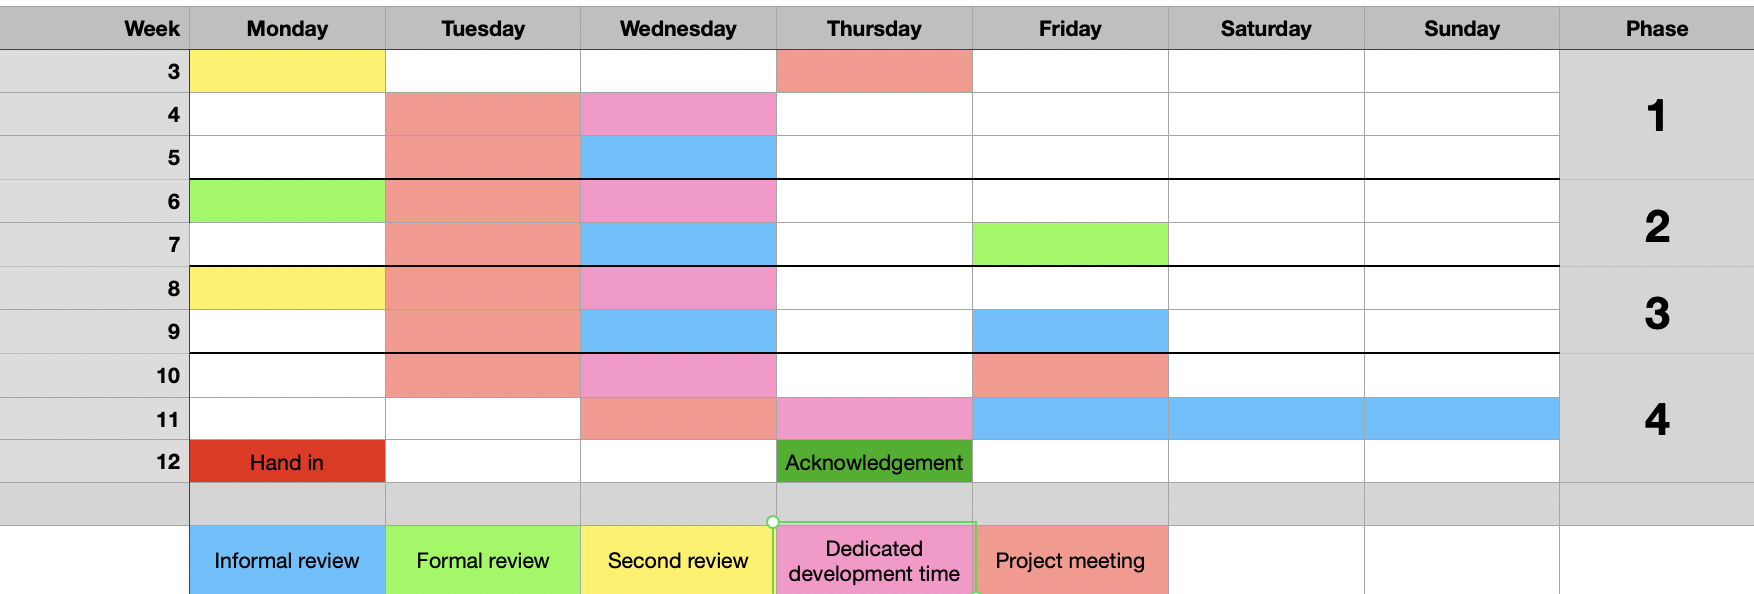
\includegraphics[width=\linewidth]{images/schedule_after.png}
              \caption{Schedule from SDP, showing when each baseline was reached.}\label{fig:schedule}
            \endminipage\hfill
        \end{figure}
      
      \subsection{Version Control \& Configuration Management \label{cm}}
        The decision to use git as version control was taken during phase 1
        and it worked quite well. The few issues that we did have were small and easy to deal with.
        To educate the group, PG held a 45 minute long education of basic usage of git which was also
        recorded so that members that missed it could watch afterwards.
        \\ \\
        While git was used to update files, E-PUSS was used to track the version numbers
        of the documents. These were recorded in the Status Reports.
        \\ \\
        One thing that differed from the initial plan of git usage was when updating
        the version of a document that had reached baseline. For this to work efficiently,
        a \emph{patch} branch was created which forked from the \emph{development} branch.
        The updated document was then put into the \emph{patch} branch which then got merged
        to \emph{master}. This process took a little longer, but seemed like a solid solution that kept the \emph{master} branch up to date, and secure.
        \\ \\
        Figure \ref{fig:commits_total} and \ref{fig:commits} illustrates the commit distribution
        and commit history during the project. As of writing this report, a total of 18 out of 21 group memebers have commited to the github repository with a total of 1,139 commits.
        
        \begin{figure}[!htb]
            \minipage{0.16\textwidth}
            \endminipage\hfill
            \minipage{0.32\textwidth}
              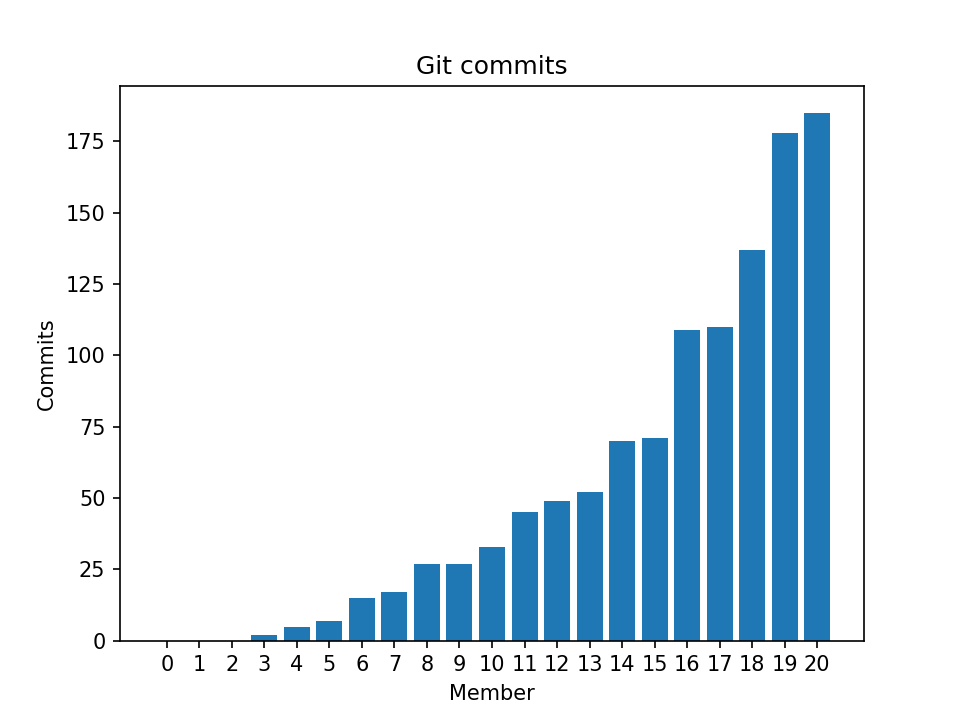
\includegraphics[width=\linewidth]{images/commits.png}
              \caption{Commit distributed throughout the group.}\label{fig:commits}
            \endminipage\hfill
            \minipage{0.32\textwidth}
              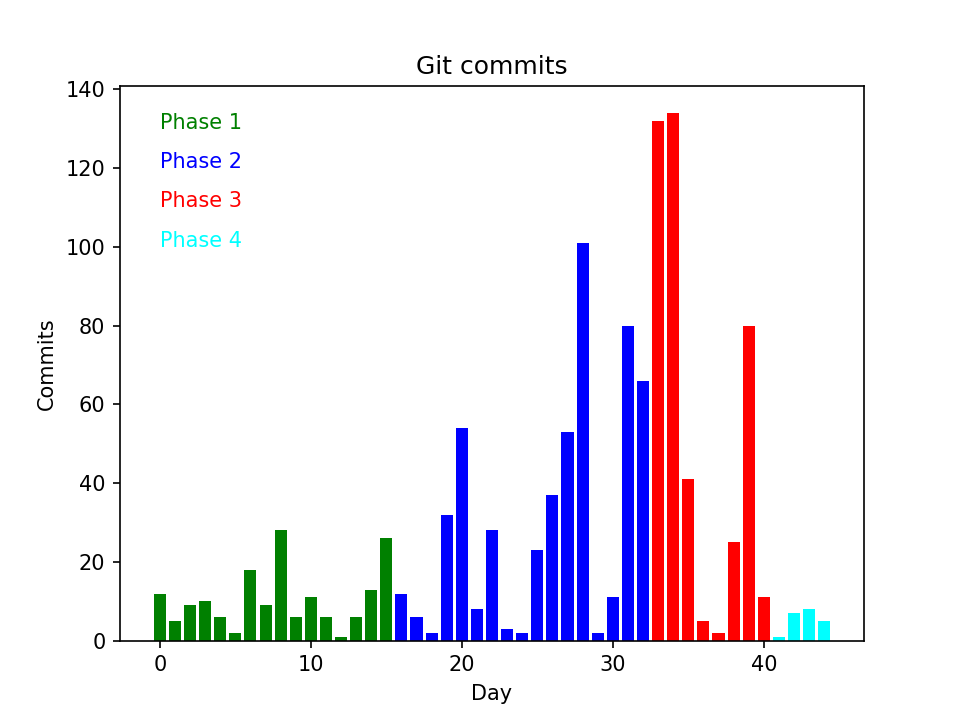
\includegraphics[width=\linewidth]{images/commits_total.png}
              \caption{Commits for each phase.}\label{fig:commits_total}
            \endminipage\hfill
            \minipage{0.16\textwidth}
            \endminipage\hfill
        \end{figure}

    \subsection{Status \& Problem reports}
        13 problem reports were reported during the lifetime of the project. All of the reports
        resulted in an update of the documents which lead to an update of the status reports.
        However, some of the problem reports were logically connected and thus only resulted
        in a single update in the status reports.
        \\ \\
        As seen in figure \ref{fig:versions} most documents did not require more than one or two changes
        after baseline was reached. Documents for phase 4 is not included in the figure since none of the documents for the phase are in baseline as of writing this report.
        
        \begin{figure}[!htb]
            \centering
            \minipage{.32\textwidth}
              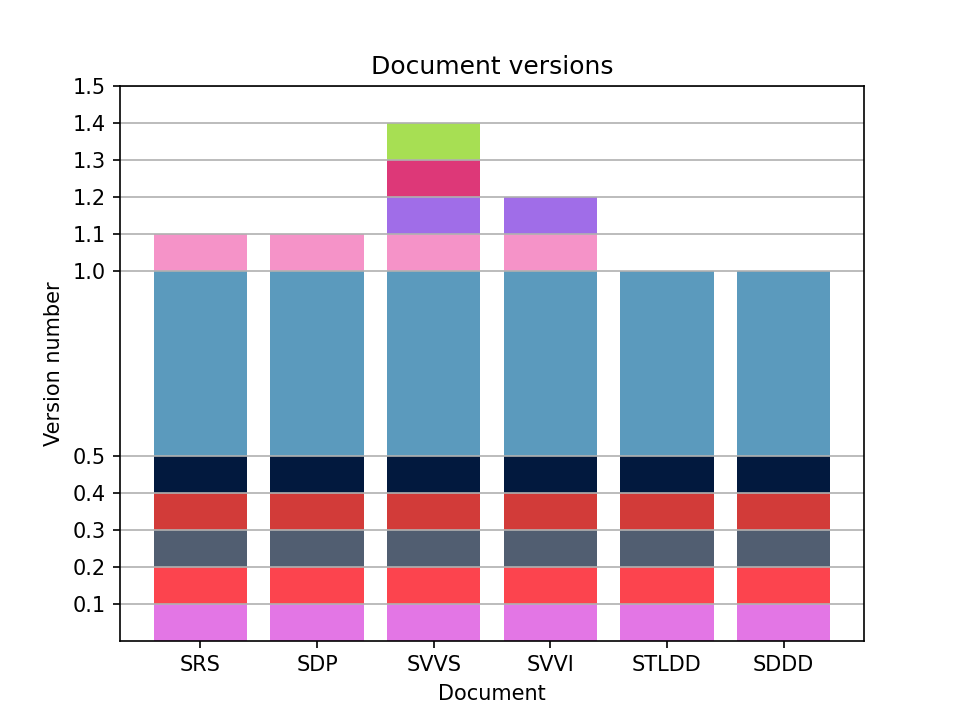
\includegraphics[width=\linewidth]{images/document_versions.png}
              \caption{Document version numbers from phase 1-3}\label{fig:versions}
            \endminipage\hfill
        \end{figure}
        
    \subsection{Online Communication \label{communication}}
        After the first project meeting (held on Zoom) the decision to move to
        Discord was taken. For the remainder of the project Discord served as the only communication channel
        and worked flawlessly.
        \\ \\
        However, while the online communication worked very well for the most part, it resulted
        in a lack of connection between group memebers. For instance, even though two of
        the ground rules specified in SDP were to actively participate during meetings,
        and, as much as possible have the camera on, this did not happen.
        The majority of the time during the project group meetings was
        spent as a monologue from the president with a handful of cameras on.
        When discussions occured it was mostly the same people who spoke, which resulted
        in about 15 people not saying a word during the entire meeting.
        This caused frustration as it was difficult to gauge the response of the group. 
    
    \subsection{Running the system locally \label{system_locally}}
        Getting the system to run locally caused more issues than expected and even late
        into phase 3 there were several members who's local servers would'nt run.
        To aid people with this, a cheat sheet was created which included step by step
        instructions how to get the system running. Though it is unknown if and how
        much this helped, it seemed like a natural and reasonable solution.
        

\section{Analysis \label{analysis}}
    This section desribes our perception of how the project went and how it lined up with our expectations. 
    This section follows the same structure as the Project Overview.

    \subsection{Phase 1. Week 3-5} 
        The first informal review, the bulk of the remarks consisted of grammatical errors, rather 
        than flaws in the  content. To correct for this, we introduced a guiding document that was 
        supposed to aid reviewers. The idea of this document was to be a reference for all future reviews, and 
        thus cointained information about reviewing code that would have to be filtered out when 
        reviewing a docuement and vice versa. The document did help to some extent, since the next 
        batch of reviewers had quite a few more useful remarks. Not to say that correct grammar and 
        spelling isn't important, content is simply more important. 
        \\ \\
        The influx of usefull remarks exposed another flaw in our review process. The inital plan was 
        that each reviewer presented their remarks, which would then be either accepted or discussed further. 
        The reference document had failed to mention how a reviewer would go about organizing their 
        remarks, which led to poorly structured presentations and discussions that were hard to follow. 
        \\ \\
        To ensure the quality of future reviews we threw out the reference document and took a simpler 
        approach that borrowed heavily from the format of the formal reviews. Reviewers got a review 
        guide that was specific to the item being reviewed and all remarks were filled into a simple 
        table that was then sent to the authors of the document before the meeting. During the review meeting, 
        only remarks that warranted discussion were mentioned and all other remarks were fixed. This 
        procedure was kept during the rest of the project and it worked very well. 
        \\ \\
        We also focused on improving the work distribution and staying on schedule. The following list 
        describes the measures we took: 
        \begin{itemize}
            \item Increase the scheduled work shifts from 1 to 2 per week.
            \item Have PG engage more with the groups, instead of relying on group leaders to act as a 
            bridge between management and other members. 
            \item Redistribute tasks from PG to SG and TG. 
        \end{itemize}
        
    \subsection{Phase 2. Week 6-7}
        There is not a lot to be said about the second phase. A lot of what had made the first phase difficult 
        was ironed out during the transition. Group members where getting more comfortable with their roles and 
        the tools we used. 
        
    \subsection{Phase 3. Week 8-9 \label{analys_phase3}}
        As explained in section \ref{phase3} this phase became quite stressful and 
        was a week late to reach baseline. The reason behind the stress and delay was
        probably a combination of the following:
        \begin{itemize}
            \item Important and time-consuming activites in other courses.
            \item Poor understanding of how the system was actually suppose to be work and
                    put together.
            \item Lack of communication between the groups in DG which resulted in 
                    extra work, such as different variable names between frontend/backend.
            \item SG feeling unsure what to do which meant that important workforce was missed.
                    Figure \ref{fig:week8} and \ref{fig:week9} clearly illustrates this as
                    SG only spent an average of 7 hours while DG spent 17 hours on average.
            \item Uncertainties in SRS, which resulted in certain ambiguities regarding requirements for the 
                    system. For instance, certain design choices were either not specified or not
                    specific enough which resulted in that DG had to improvise.
            \item Lack of knowledge and experience with the technologies, which meant that valuable time
                    was spent on doing research on how certain technologies or frameworks work (like jsp, tomcat etc). This should have been done earlier in the project so that phase 3 could
                    be entirely about implementing the STLDD instead of googling.
            \item The waterfall method is not suited for a project when the group has little to zero          experience with the technology. Because of this, we believe that an agile development         method would be more suitable for this project.
        \end{itemize}
    
    \subsection{Phase 4. Week 10-11}
        This phase was very straightforward and by the time phase 3 reached baseline, the group was
        comfortable and knew their roles. The majority of SSD and SVVR were already finished which
        meant that it went without issues. Though we must note that the writing of this document
        is done in phase 4 so it is not oficially over yet.

    \subsection{Reported Time}
        While the group did agreed early to not have heros in the project, they did occur anyways.
        Unfortunately we believe that this is unavoidable and a natural result of working in a big group of people
        in a school project. We motivate this rather cynical statement with the fact that people take school more or less serious and have different goals and ambitions. If a group with three students where student A and B
        aims to learn as much as possible and are ready to work 10 hours a week, while student C only wants to
        pass the course and is not ready to put more than 5 hours a week, the hereos will show up and 
        some people will do less.
        \\ \\
        This was not unexpected and in fact, something that PG pointed out very early on. On several occasions
        members were encouraged to talk about their goals and ambitions so they would get an understanding
        of what to expected from each other. Wether this had an impact or not is unknown but we felt that there was not much more to do.
    
    \subsection{Keeping Schedule}
        We believe that the schedule was kept with minor deviations, but we did underestimate the time
        to reach a baseline. We believed that baseline would be reached straight after formal review, without any marks. This turned out to be quite naive since none of the formal reviews resulted in baseline without \emph{any} adjustments required. 
        \\ \\
        Several members argue that more time should have been spent during phase 3 and
        this was in fact the initial plan. However, after a dicussion, the group \emph{did} take
         the decision to have two weeks for phase 3. While more time during phase 3
        obviosuly would make it less stressful, one can argue that the reason it was stressful
        was not because of lack of time, but rather because of poor communcation between the groups,
        poor preparation and the rest of the possible reasons mentioned in section \ref{analys_phase3}. Also, if more time would be spent on phase 3, the time has to come
        from somewhere, for instance phase 2, but then there would be less time to do the planning.
        Thus we propose the following improvements if we would do the project again:
        \begin{itemize}
            \item PG should be more strict from the beginning and be \emph{very} clear what each group
                    should do and what their responsibilities are. 
            \item DG should choose their groups during the first week so that they can start to work
                    and do research as soon as possible.
        \end{itemize}

    \subsection{Version Control \& Configuration Management}
        As explained in section \ref{cm} there were 3 members that did not do a single
        commit to the project repository. While the cause of this is unknown we consider
        one of the following explanations:
        \begin{enumerate}
            \item They do not know how to use git.
            \item They have worked in groups and thus not needed to commit anything themselves.
            \item They have not participated to the project.
        \end{enumerate}
        As we will not investigate this any further we do believe that it would have been
        better if every member was forced to do several pushes to the repository as soon
        as the decision to use git was taken. This would reduce the chances that people
        do not know how to use the tool and thus eliminate option 1. 
        \\ \\
        As a side not we would also like to mention that version control systems like git
        should be introduced in our education, since they are such a vital part of 
        software engineering.
    
    \subsection{Status \& Problem reports}
        Even though the UI of E-PUSS seems to be form the 90's, the functionality worked
        pretty well for creating problem reports and handling status reports.
        Even though git has support for both of these, the amount of work and time to ensure
        that everyone gets the education required to use it seemed not worth it and thus
        we believe that it was the right decision to use E-PUSS.
    
    \subsection{Online Communication}
        The biggest benefit of online communication was that it was very easy and quick to
        contact people and to share files, join different rooms etc. It was also easier for
        people to participate during meetings since no travelning was required.
        However, as described in \ref{communication} the lack of participation and active cameras
        hade a negative impact on the communication.
    
    \subsection{Running the system locally}
        To reduce problems to get the system running locally, 
        we conclude in the following possible solutions:
        \begin{enumerate}
            \item Set a deadline for everyone to get the system running locally. 
                    A list could be used so that each member can sign when they have
                    the system running as well as a help list if they need guidance.
                    This would force people to get the system running and PG and SG
                    would notice who had not.
            \item While out of our hands, the laboratories in the course should be introduced earlier.
        \end{enumerate}
        
    \subsection{Group Managers}
        Besides the project managers, we appointed a manager for each work group SG, DG and TG. The tasks of the system manager and test manager were outlined in the Project Instructions and were quite clear, but the role of devolpment manager was not specified and thus \emph{not} clear.
        This resulted in the some ambiguities for the development manager regarding what the responsibilites and what purpose the role served. This also lead to certain tasks falling between the cracks or 
        delayed, such as splitting DG intro groups, telling inner groups in DG what to do etc.
        \\ \\
        We believe that this could have been prevented by carefully specifying the responsibilites of the
        role in the beginning of the project and having a stronger conversation the person who had the role.
        Another option would be to \emph{not} have a development manager
        and instead give the responsibilities to SG. This could also result in the role and purpose of 
        SG more clear, which as discussed in \ref{analys_phase3} was a problem during phase 3.
        
\section{Six tips for future project groups \label{tips}}

    To help future project groups we have acquired five tips that we would like to share.
    They come as a result of the project and the lessons we have learned.
    
    \subsection{Tip 1}
        In the beginning, ensure that you spend enough time to fully understand the purpose and the 
        responsibility for each role. Spending more time on this early on will be useful as the project
        proceeds as it will help to ensure that everyone knows what to do, and what their responsibilites are. It is also important to convey this information to the groups.
        
    \subsection{Tip 2}
        Since this semester has four courses running in parallel, it could be a nice idea
        to book times for the group to not only for work on the project, but also to study
        for other courses. This could improve the teambuilding and communication within the
        group and ensure that people do not fall behind in other courses.
    
    \subsection{Tip 3}
        Ensure that you know what you want to review during the informal reviews. The following
        questions can be used:
        \begin{enumerate}
            \item \emph{Who} is reviewing
            \item \emph{What} should the revieweer look for
            \item \emph{Where} should the comments/notes from the reviewer be, and in what format
        \end{enumerate}
        Also remember that the informal reviews are meant to catch errors and \emph{improve}
        the documents. It is pointless to have a review if everyone just agrees and finds nothing. 
        We believe it is better to be \emph{too} hard than too gentle.
        
    \subsection{Tip 4}
        Just like any other programming project, development time is very hard to estimate. 
        The third phase was by far the most stressful due to optimistic planning and delays caused by earlier phases. 
        When making a schedule for a future project, it would be wise to give development as much time as possible and 
        take into account that things does not work out of the box.
        
    \subsection{Tip 5}
        Use each phase as a learning experience, be open to alter your procedures based on feedback from the group, \emph{even if} it requires making changes to baselined documents.
        
    \subsection{Tip 6}
        Spend time to actively ask and talk about feedback.
        
        Feedback does not come on its own however, you will actively have to talk to your group members to identify issues. 
    
\section{Conclusion \label{conclusion}}
    An important thing to consider is the external stress factor that other courses, and seperate 
    modules of this course, introduced. It has been a shared sentiment within the group that the 
    work load during this semester has been overwhelming. Several group members have had issues 
    balancing school work, some even putting other courses on hold. Whilst it is expected of a 
    student who studies at full pace to put 40 hours/week into their school work, the reality 
    of the situation is that most do not. The the sudden jump in time required had a big impact 
    on the stress level felt by the group. Despite this, the group came togheter and worked hard to get results. 
    \\ \\
    TimeMate was delivered on time and all the major requirements were met. By this metric it would be 
    fair to say that the project went well. There are multiple lessons to learn from this, which are 
    very welcome. As preparation, as well as during, the writing of this report the group discussed the project. The perception within the group is that the project was fun and very valuable from an academic standpoint. So in conclusion, the members of project group 2 are proud of their collective effort and consider 
    this project to have been a rather stressful, but equally valuable, experience. 
    
\newpage
\section{Acknowledgements}
    Thank you to Christine Lindholm for you guidance and patience. \\ \\
    Thank you to Emelie Engström for making making our documents legible. \\ \\
    Thank you to Anders Bruce for your technical expertise. \\ \\
    Lastly, a big thank you to every member in group 2:
    \begin{itemize}
        \item Victor Krook (PG)
        \item Assar Orpana (PG)
        \item David Vilppu (SG Leader)
        \item Ramtin Mosavi (SG)
        \item Filip Sjövall (SG)
        \item Mustafa Elomeiri (SG)
        \item Alexandra Galonja (DG)
        \item Anna Bergvall (DG)
        \item Annelie Sinander (DG)
        \item Hjalmar Janson (DG)
        \item Oscar Johansson (DG Leader)
        \item Sebastian Forslund (DG)
        \item Abd Salam (DG)
        \item Alaa Wahbah (DG)
        \item Alexander Olofsson (DG)
        \item Johan Wulf (DG)
        \item Alexander Möhle (TG Leader)
        \item Lazar Trpeski (TG)
        \item Max Palmgren (TG)
        \item Malte Wallander (TG)
        \item Anas Abu Al-Soud (TG)
    \end{itemize}

\end{document}
